% FastLane progress report -- ACL-style layout, single column.
% Build: cd report && pdflatex fastlane_report && bibtex fastlane_report && pdflatex fastlane_report && pdflatex fastlane_report
\documentclass[11pt,a4paper]{article}

\usepackage[T1]{fontenc}
\usepackage[utf8]{inputenc}
\usepackage{times}
\renewcommand{\ttdefault}{lmtt}
\usepackage{microtype}
\usepackage[a4paper,top=2.5cm,bottom=2.5cm,left=2.5cm,right=2.5cm]{geometry}
\usepackage{graphicx}
\usepackage{booktabs}
\usepackage{tabularx}
\usepackage{longtable}
\usepackage{array}
\usepackage{amsmath}
\usepackage{xcolor}
\usepackage{url}
\usepackage[small,labelfont=bf]{caption}
\usepackage{tikz}
\usetikzlibrary{positioning,arrows.meta,fit}
\PassOptionsToPackage{hyphens}{url}
\usepackage[hidelinks]{hyperref}
\newcommand{\hcell}[1]{\begin{tabular}[b]{@{}r@{}}#1\end{tabular}}  % right-aligned two-line table header

% ACL-like headings: section \large bold, subsection \normalsize bold, paragraph run-in bold.
\makeatletter
\renewcommand\section{\@startsection{section}{1}{\z@}{-2.2ex plus -0.5ex minus -0.2ex}{1.1ex plus 0.2ex}{\large\bfseries\raggedright}}
\renewcommand\subsection{\@startsection{subsection}{2}{\z@}{-1.8ex plus -0.5ex minus -0.2ex}{0.8ex plus 0.2ex}{\normalsize\bfseries\raggedright}}
\renewcommand\paragraph{\@startsection{paragraph}{4}{\z@}{1.2ex plus 0.5ex minus 0.2ex}{-1em}{\normalsize\bfseries}}
\makeatother
\setlength{\parindent}{1em}
\setlength{\emergencystretch}{2em}
\setlength{\parskip}{0pt}
% Let several floats share a text page so tables stay near their text instead of piling up at the end.
\renewcommand{\topfraction}{0.85}\renewcommand{\bottomfraction}{0.6}\renewcommand{\textfraction}{0.1}
\renewcommand{\floatpagefraction}{0.75}\setcounter{topnumber}{3}\setcounter{bottomnumber}{2}\setcounter{totalnumber}{5}
\makeatletter\setlength{\@fptop}{0pt}\setlength{\@fpsep}{10pt plus 2pt}\makeatother  % float pages start at the top
\setlength{\textfloatsep}{10pt plus 2pt minus 2pt}
\setlength{\floatsep}{8pt plus 2pt minus 2pt}
\setlength{\intextsep}{8pt plus 2pt minus 2pt}
\renewcommand{\arraystretch}{1.1}
\newcolumntype{L}{>{\raggedright\arraybackslash}X}
\newcommand{\cmd}[1]{{\small\ttfamily\def\_{\textunderscore\allowbreak}#1}}  % code names may break after "_"
\newcommand{\Rs}{Rs~}
\let\olditemize\itemize
\renewcommand{\itemize}{\olditemize\setlength{\itemsep}{1pt}\setlength{\parskip}{0pt}\setlength{\topsep}{2pt}}

\title{\Large\bfseries FastLane: A Voice Agent That Uses a Small Model for Easy Turns\\
and a Large Model Only for Hard Ones\\[4pt]
\normalsize\normalfont LMA Group Project 2026 --- Mid-Submission Report (30 October 2026)}
\author{
  \textbf{Team: Chaturvedi and Sons}\\[4pt]
  \begin{tabular}{c@{\hspace{3em}}c@{\hspace{3em}}c}
  \textbf{Noel Alex Jacob} & \textbf{Aviral Tyagi} & \textbf{Sankalp Chaturvedi}\\
  2025201085 & 2025201086 & 2025201083\\[4pt]
  \multicolumn{3}{c}{\textbf{KSPSVLN Siddardha Kumar Kavuri}}\\
  \multicolumn{3}{c}{2025201061}
  \end{tabular}\\[6pt]
  {\small GitHub: \url{https://github.com/Sankalp0109/FastLane-Adaptive-Voice-Agent}}
}
\date{}

\begin{document}
\maketitle
\vspace{-1.2em}

\begin{abstract}
\noindent FastLane is a phone agent that books, changes and cancels movie tickets, bus tickets and restaurant tables for
Indian-English callers. A LoRA-tuned Qwen2.5-3B answers every turn first and passes only hard turns to a large API
model (gpt-oss-120b) or to staff; every action goes through a tool and policy gateway that enforces booking rules
and a read-back confirmation in code. This report describes everything built so far: a deterministic practice
booking system with 11 tools, a 360-call test set with a simulated caller, a data generator that runs an oracle agent
through the real orchestrator, five data versions and five Kaggle training sessions, and a local voice pipeline (Silero
VAD, Whisper, Kokoro). Offline, the tuned small model routes 99.3\% of held-out steps correctly (untuned: 89.1\%) and
fills tool arguments exactly in 99.0\% (untuned: 26.8\%). On 24 end-to-end calls, FastLane with the fixes found in
the pilots succeeds in 95.8\% of calls, against 87.5\% for the large model alone (B1), 95.8\% for the large model
used as a router (B3) and 29.2\% for the untuned small model alone (B2). It needs 80\% fewer large-model calls than
B1 and makes no unconfirmed or duplicate bookings, while B1 makes them in 8 of 24 calls. FastLane is not faster: the large model on
Groq answers a turn in 1.17\,s (p95 2.3\,s), while the local 3B model needs 1.55\,s (p95 7.6\,s), so the latency
hypothesis fails on this hardware. The ablations support two more hypotheses: without date and alternative tools
(A2) the large model is called about twice as often, and with rules only in the prompt (A3) 13 of 24 calls make a
booking change the caller never confirmed. On real Indian-English speech
(Svarah), Sarvam's recogniser has the lowest error (5.8\% WER vs.\ 9.5--10.5\% for Whisper), and a TTS$\rightarrow$STT
round trip shows that recogniser noise roughly triples the tuned model's argument errors (98.1\% $\rightarrow$ 94.3\%
exact). We report each iteration with the reason it was needed, and what remains for the final comparison.
\end{abstract}

% =====================================================================================================================
\section{Introduction}

A voice agent has about a second to reply before callers talk over it or repeat themselves. Most agents send every
turn to a large API model, which adds 1--3\,s per turn and costs too much for a small cinema, bus operator or
restaurant. Yet most turns in a booking call are easy (a date, a seat count, a name, a ``yes'' to a read-back); only
a few are hard (``next Friday'', a sold-out show, a caller changing their mind, a request that breaks a rule). A wrong
booking is worse than a slow one, and recognisers often mishear Indian names, places and numbers. Our question is
\emph{for each turn, which model should reply}, judged on speed, correctness and safety together.

The proposal states three research questions: (RQ1) can a LoRA-tuned small model that both answers easy turns and
decides when to pass a turn on cut time per turn by $\geq$50\% without a real drop in booking success compared with a
large-model-only agent; (RQ2) does moving rules and routine work (dates, alternatives, policy checks) from the prompt
into code reduce large-model calls and unsafe bookings; (RQ3) does a small model trained only on movies and buses
still work on restaurants. They come with seven hypotheses (Table~\ref{tab:hyp}).

\paragraph{Progress and structure of this report.} Table~\ref{tab:progress} summarises progress by phase of the
plan: Phases 0--7 are done, and Phase 8 (the full comparison) has started with baseline and ablation runs on a
24-call sample. The report follows the mid-submission items: the system (Section~\ref{sec:system}), datasets
(Section~\ref{sec:data}), baselines, ablations and metrics (Section~\ref{sec:eval}), training
(Section~\ref{sec:training}), results of all experiments run so far (Section~\ref{sec:results}), challenges and
mitigation (Section~\ref{sec:lessons}), the status of each hypothesis (Section~\ref{sec:status}) and the remaining
work with a timeline to the final submission on 15 November (Section~\ref{sec:todo}). All code is in one Python
package (about 10.5k lines in \cmd{src/fastlane}, 203 passing tests) on GitHub, with the Kaggle notebook, result
files and a run log recording every experiment.

\begin{table}[tbp]
\centering\small
\begin{tabularx}{\linewidth}{@{}>{\raggedright\arraybackslash}p{4.0cm}>{\raggedright\arraybackslash}p{2.3cm}L@{}}
\toprule
Phase & Status & What exists \\
\midrule
0 Scaffolding & done & Python package, CLI (\cmd{fastlane \dots}), 203 tests \\
1 Practice world & done & SQLite booking system for 3 domains, fixed seed, snapshot/restore per call \\
2 Gateway and booking record & done & 11 tools, rules in code, read-back gate, identity check, error injection, 2 rules added after pilots \\
3 Retrieval & done (corpus partial) & BM25 over 25 policy documents, old/new policy versions, early lookup; Recall@3 0.967 \\
4 Models and orchestrator & done & all 12 systems run end to end; large model with rate-limit backup \\
5 Evaluation harness & done & 360-call test set, LLM caller, resumable runner, all proposal metrics \\
6 Training & v1--v3 and v5 trained & 5 data versions, 6 Kaggle sessions; v3: route 99.3\%, arguments 99.0\% offline; v5 more robust to recogniser noise \\
7 Speech & done & browser voice demo, STT comparison on Svarah, TTS$\rightarrow$STT noise for training \\
8 Experiments & started & FastLane, B1, B2, B3, A2, A3, A8 on 24 calls (A1 from the pilot); larger runs limited by API quota \\
\bottomrule
\end{tabularx}
\caption{Progress by phase of the project plan.}
\label{tab:progress}
\end{table}

% =====================================================================================================================
\section{Related Work}

Model routers such as FrugalGPT (a cascade of LLMs of increasing cost) and RouteLLM (a router trained on
preference data) choose one model per \emph{question} on single-turn benchmarks. FastLane routes \emph{per turn}
inside a long, tool-using dialogue, and the router is the small model itself, so easy turns pay no routing delay.
Tool-agent benchmarks such as $\tau$-bench check the final database state with a simulated user, which we adopt, but
do not measure latency, so they reward always using the largest model; we report speed, success and unsafe actions
together. We tune Qwen2.5-3B-Instruct with LoRA on a 4-bit base (QLoRA) and serve it with MLX; the speech layer uses
Silero VAD, Whisper, Sarvam's Indian-language recogniser and Kokoro TTS.

% =====================================================================================================================
\section{System}\label{sec:system}

\begin{figure}[tbp]
\centering
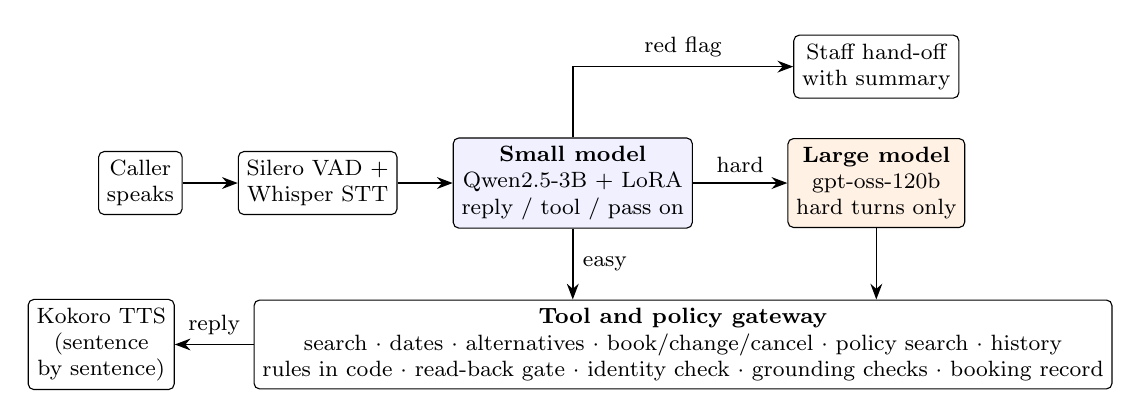
\begin{tikzpicture}[font=\footnotesize, node distance=6mm and 7mm,
  box/.style={draw, rounded corners=2pt, align=center, minimum height=8mm, inner sep=3pt, fill=white},
  arr/.style={-{Stealth[length=2mm]}, semithick}]
\node[box] (caller) {Caller\\speaks};
\node[box, right=of caller] (stt) {Silero VAD +\\Whisper STT};
\node[box, right=of stt, fill=blue!6] (small) {\textbf{Small model}\\Qwen2.5-3B + LoRA\\reply / tool / pass on};
\node[box, right=12mm of small, fill=orange!10] (large) {\textbf{Large model}\\gpt-oss-120b\\hard turns only};
\node[box, above=5mm of large] (staff) {Staff hand-off\\with summary};
\node[box, below=9mm of small, xshift=14mm] (gw) {\textbf{Tool and policy gateway}\\ search $\cdot$ dates $\cdot$ alternatives $\cdot$ book/change/cancel $\cdot$ policy search $\cdot$ history\\
rules in code $\cdot$ read-back gate $\cdot$ identity check $\cdot$ grounding checks $\cdot$ booking record};
\node[box, left=10mm of gw] (tts) {Kokoro TTS\\(sentence\\by sentence)};
\draw[arr] (caller) -- (stt);
\draw[arr] (stt) -- (small);
\draw[arr] (small) -- node[above]{hard} (large);
\draw[arr] (small.north) |- node[pos=0.75, above]{red flag} (staff.west);
\draw[arr] (small) -- node[right]{easy} (gw.north -| small);
\draw[arr] (large.south) -- (gw.north -| large);
\draw[arr] (gw) -- node[above]{reply} (tts);
\end{tikzpicture}
\caption{FastLane. Every caller turn goes to the tuned small model, which replies (optionally with a tool call),
passes the turn to the large model, or hands it to staff. Neither model writes to the booking system directly.}
\label{fig:arch}
\end{figure}

\paragraph{Practice world.} One SQLite database built from a fixed seed with a fixed ``now'' (Thursday 15 October
2026, so Dussehra and Diwali fall inside the booking window): 4 cinemas, 12 screens, 9 films and 1,440 shows with
seat maps (41,110 seats taken); 6 bus routes between Hyderabad and Bengaluru, Vijayawada and Chennai with 720 trips
(6,966 seats taken); 3 Tandoor Tales branches with 45 tables and 2,613 existing reservations; 200 callers with 510
past bookings (for returning callers) and 70 open bookings. Some shows, trips and slots are sold out on purpose for
the ``needs an alternative'' calls. Each test call starts from a snapshot of the same database.

\paragraph{Gateway and rules.} The gateway exposes eleven tools with validated arguments:
\cmd{search\_inventory}, \cmd{resolve\_date}, \cmd{find\_alternatives}, \cmd{create\_booking}, \cmd{modify\_booking},
\cmd{cancel\_booking}, \cmd{lookup\_booking}, \cmd{get\_caller\_history}, \cmd{search\_policy}, \cmd{send\_sms} and
\cmd{handoff\_to\_staff}. Rules are enforced in code, not in the prompt:
at most 10 movie tickets and changes up to 4\,h before the show; at most 6 bus seats, name/age/gender for every
passenger, refunds of 90/75/50/25\% by hours to departure; restaurant party limits (12/10/8 by branch) and a deposit
for large groups. A create, change or cancel first returns a read-back that must be spoken to the caller; the same
call succeeds only after the caller confirms it in the next turn. Changes need the phone number of the booking.
Four rules were added after observed failures (Section~\ref{sec:impl}): \emph{passenger source} (every bus
passenger's name and age must have been said by the caller or come from their history, and the passenger count must
cover the seats asked for), \emph{grounding} (the booked venue and time must have been said by the caller or offered
by the agent earlier in the call), \emph{heard count} (a ticket count or party size must be a number the caller said)
and \emph{origin heard} (a bus search from a city other than Hyderabad needs the caller to have named it). There is no payment tool; SMS is only logged.

\paragraph{Booking record and retrieval.} A typed per-domain record (film/route/branch, date, time, count,
passengers, name, read-back status) is shared by both models and the staff summary. Policy questions use a BM25
index over 25 policy documents (fares, refund rules, FAQs, allergen-tagged menus, a
festival calendar, an old and a current version of the bus refund policy); a lookup starts on partial transcripts
and is reused if the final transcript matches (early lookup).

\paragraph{Routing.} The small model outputs one JSON object: \cmd{route} (self / llm / staff), the slots heard this
turn, an optional tool call and the words to say. A turn goes to the large model when the small model routes it there
or its escalation score (from token log-probabilities) exceeds a threshold, and in code on a tool error, no
availability, a changed earlier choice, an unconfident policy match, a repeated tool call, and (added after
failures) a policy answer with numbers or a ``no'' answer after a policy search, a refund or fee figure given with no
search, or a reply that claims a booking change the gateway did not make. It goes to staff on the small model's ``staff'' route or two failed tool calls in a row. The large model gets
the booking record, the last turns and the same tools, finishes the turn, and returns control. Read-back confirmations
and goodbyes are templates that need no model call.

\paragraph{Models and serving.} Large model: \cmd{openai/gpt-oss-120b} on Groq (free tier during development, paid
tier with no backup for the final runs), during development with \cmd{gemini-3.5-flash} as a backup when Groq would make a call wait more than 10\,s (capped at 20\,s, no retry);
every response records which model answered, and rate-limit waiting is logged separately (\cmd{throttle\_ms}) and
never counted as model time. Simulated caller: Qwen2.5-7B, local. Small models, tuned and untuned, run as 4-bit MLX
models (1.6\,GB) on a 16\,GB Apple M4 behind an OpenAI-compatible server that returns log-probabilities, so both are
timed on the same stack.

% =====================================================================================================================
\section{Implementation Details}\label{sec:impl}

\paragraph{Code base.} FastLane is one Python package (about 10,600 lines in \cmd{src/fastlane}) with one command-line
tool, \cmd{fastlane}, and 211 unit tests (about 1,700 lines) that run in 18\,s without any model or network, using
scripted model clients. Every long job is resumable: an evaluation run skips calls already in its results file, the
speech round trip caches every clip, and training finishes from a saved adapter. Every run, failure and change is
logged with its evidence in \cmd{docs/EXPERIMENT\_LOG.md} (27 sections) and \cmd{results/}.
Table~\ref{tab:modules} lists the parts.

\begin{table}[tbp]
\centering\small
\begin{tabularx}{\linewidth}{@{}l>{\raggedright\arraybackslash}p{0.27\linewidth}L@{}}
\toprule
Package & What it does & How (main choices) \\
\midrule
\cmd{world} & practice world & SQLite schema and a seeded generator (fixed ``now'', planned sold-out cases, 200 callers with history); seat maps for cinemas and sleeper/seater buses \\
\cmd{gateway} & the only way to the data & 11 tools with typed arguments (pydantic); rules, read-back gate, identity check and grounding checks in code; spoken-date resolver; fuzzy matching of names said over the phone; the shared booking record \\
\cmd{agent} & orchestrator & per-turn routing (small $\to$ large $\to$ staff), escalation triggers in code, templates for read-backs, confirmations and goodbyes, a timed trace of every turn \\
\cmd{models} & model clients & one OpenAI-compatible client for Groq, Gemini, Ollama and MLX (rate-limit headers, \cmd{throttle\_ms}, backup model); prompts; parser for the small model's JSON; escalation score from log-probabilities \\
\cmd{retrieval} & policy search & BM25 index over 25 policy documents; early lookup on partial transcripts; 67-question retrieval test \\
\cmd{training} & practice calls and fine-tuning & rule-based caller and agent produce training steps through the real gateway; speech noise (rules, later TTS$\to$STT round trip); Kaggle QLoRA notebook; local merge and 4-bit MLX conversion; offline step check \\
\cmd{eval} & experiments & 360 scripted test calls, simulated caller (Qwen2.5-7B), scorer (outcome, hand-off, answer), metrics (success with Wilson CI, p50/p95, router recall, unsafe writes), reports and plots \\
\cmd{speech} & voice demo & browser page and WebSocket server: Silero VAD, Whisper large-v3-turbo (MLX) with a domain word list, the same agent, Kokoro TTS sentence by sentence; WER tools for the STT comparison \\
\bottomrule
\end{tabularx}
\caption{Packages of the implementation.}
\label{tab:modules}
\end{table}

\paragraph{How changes were made.} Every fix below started from an observed failure (a crashed run, a failed test
call, a voice-demo call, or a wrong offline step), was written as a unit test first where possible, and was then
checked against the generated training data: after each gateway rule, all 650 practice calls were regenerated through
the new code to confirm that the rule never blocks a correct booking (every time: no training example changed), so
no retraining was needed for code fixes. Fixes to the agent were never applied in the middle of a comparison run; a
fixed system is reported as a separate run.

\paragraph{Everything fixed so far.} Table~\ref{tab:allfixes} lists every fix in order, with the problem that led to
it, how it works, and its effect. Rows 1--10 concern infrastructure and training, rows 11--37 the agent, the gateway,
the data and the evaluation.

{\small
\setlength{\tabcolsep}{4pt}
\begin{longtable}{@{}r>{\raggedright\arraybackslash}p{0.07\linewidth}>{\raggedright\arraybackslash}p{0.30\linewidth}>{\raggedright\arraybackslash}p{0.53\linewidth}@{}}
\caption{Every fix in the implementation so far: the problem that showed it, and what was changed. Code locations are
in the experiment log.}\label{tab:allfixes}\\
\toprule
\# & Date & Problem (where it showed) & Fix: how it works, and effect \\
\midrule
\endfirsthead
\multicolumn{4}{@{}l}{\small\emph{Table~\ref{tab:allfixes} continued}}\\
\toprule
\# & Date & Problem (where it showed) & Fix: how it works, and effect \\
\midrule
\endhead
\bottomrule
\endfoot
\multicolumn{4}{@{}l}{\emph{Infrastructure, serving and training}}\\
1 & 20 Oct & Groq free tier: 8k tokens/min; waits would inflate latency & the client reads \cmd{retry-after} and remaining-token headers and waits before sending; waiting is stored as \cmd{throttle\_ms}, never as model time \\
2 & 21 Oct & pilot hit Groq's daily limit (10--15 min waits per turn) & \cmd{FallbackClient}: a call that would wait $>$10\,s goes to \cmd{gemini-3.5-flash}; every reply records which model answered; tool history is rewritten as text for Gemini, which needs its own \cmd{thought\_signature} \\
3 & 25 Oct & Kaggle run 1 crashed at step 1 (bfloat16 in the fp16 loss scaler) & trainable LoRA weights cast to float32, leftover bfloat16 base weights to float16; the notebook stops at the first failed step \\
4 & 25 Oct & adapter merge failed on Kaggle (\cmd{torchao} vs \cmd{peft}) & \cmd{torchao} uninstalled; a failed merge no longer fails the run; merging is done locally \\
5 & 25 Oct & Ollama cannot import a LoRA-tuned Qwen2 & small models served as 4-bit MLX models by \cmd{fastlane serve} (OpenAI-compatible, with log-probabilities); the untuned base is converted the same way, so both are timed on one stack \\
6 & 26 Oct & the first ``v2'' check gave exactly v1's output & a stale merged folder was re-quantised; the merge now always starts from scratch, and weight hashes are compared before a model is evaluated \\
7 & 26 Oct & one Gemini backup reply took 45.6\,s & backup capped at 20\,s with no retry; if it fails the call waits for Groq and the lost time counts as waiting \\
8 & 28 Oct & the Kaggle run meant for data v4 trained v3 again (old dataset attached) & the notebook asserts exactly one data folder, the expected example counts and the noise type before training; v5 was then trained correctly (7 Nov) \\
9 & 9 Nov & Groq unreachable for $\sim$40 min; 4 calls told the caller ``Sorry, I didn't quite get that'' & the backup is also used for 30\,s after a connection error or a 5xx reply (not only on rate limits); other errors still raise \\
10 & 10 Nov & Gemini's free tier allows 20 requests/day; the final runs need $\sim$1,500 & final runs on Groq's paid tier with the backup switched off, so every system sees only gpt-oss-120b \\
\midrule
\multicolumn{4}{@{}l}{\emph{Pilot v0 (untuned small model), 21 Oct}}\\
11 & 21 Oct & large-model turns crashed with HTTP 400 (\cmd{gender: "female"} vs schema \cmd{M/F/O}) & lenient schema plus normalisation in the gateway; provider-side argument rejections are fed back to the model, which retries \\
12 & 21 Oct & the large model asked for passengers three times & arguments passed to write tools now fill the booking record, so details survive a refused call and a switch between models \\
13 & 21 Oct & ``Friday 23rd October'' booked on Friday 16th & an explicit day of the month beats a weekday word \\
14 & 21 Oct & \cmd{"10:00"} searched as 10 PM & ``bare hour = PM'' applies only to spoken times; two-digit \cmd{HH:MM} is literal \\
15 & 21 Oct & ``\ldots 44, male, that's all'' ended the call & a goodbye must be a short turn with no numbers \\
16 & 21 Oct & correct policy answers scored wrong (narrow no-break space in ``4 hours'') & the scorer normalises Unicode spaces and dashes; stored calls rescored \\
17 & 21 Oct & the simulated caller hung up right after ``yes'' & caller prompt: hang up only after a reference, an answer or a transfer \\
\midrule
\multicolumn{4}{@{}l}{\emph{Training data and model versions}}\\
18 & 25 Oct & v1: every remaining offline error involved a date & the small model copies the caller's own words for a date; code resolves them (\cmd{resolve\_date}, also inside search and alternatives) and stores the ISO date in the record; wrong resolutions over all 360 spoken date forms: 69 $\to$ 0. Retrained as v2 \\
19 & 26 Oct & A2 (no date tools): the date the large model worked out was lost on the next turn & the small model carries that date as \cmd{YYYY-MM-DD} in its slots; only A2 steps changed (data v3, adapter v3) \\
20 & 26 Oct & voice demo: details given together in one sentence were dropped; ``Which cinema?'' in a bus call & data v4: openings with 0--5 details in random order, 35\% without a domain word \\
21 & 27 Oct & 14.9\% of rule-based noise copies lost a detail the target still had (``four tickets'' $\to$ ``for tickets'' with quantity 4) & data v5: noise copies from a real TTS$\to$phone-channel$\to$Whisper round trip, kept only if every key detail survives \\
\midrule
\multicolumn{4}{@{}l}{\emph{Pilot v3 and the voice demo, 26--27 Oct}}\\
22 & 26 Oct & invented passenger ``Caller (40)''; 1 of 3 seats booked & \emph{passenger-source rule}: every passenger's name and age must have been said in the call (digits or words) or come from the caller's history, and the passengers must cover the seats asked for; rerun 3/3 \\
23 & 26 Oct & refund table misread (90\% instead of 25\%) & a small-model policy answer with numbers goes to the large model with the same search result \\
24 & 26 Oct & voice demo: search with a cinema nobody named, the caller's 7 PM dropped & \emph{grounding rule}: the booked venue (cinema, bus destination and non-Hyderabad origin, branch) and time must have been said by the caller or offered by the agent; the agent's own read-backs do not count \\
25 & 26 Oct & voice server: every WebSocket got HTTP 403; SQLite used from another thread & annotation import fixed; one worker thread per call \\
26 & 27 Oct & hand-off announced but no tool called; markdown read aloud; the page hid ``call ended'' & a reply that says it \emph{is} transferring hands off in the same turn; every reply is converted to plain sentences; the page waits for the last audio, then shows the transfer notice \\
\midrule
\multicolumn{4}{@{}l}{\emph{Before the final runs, 6 Nov}}\\
27 & 6 Nov & ``Authenticates'' (misheard) booked as 4 tickets & \emph{heard-count rule}: a ticket count or party size must be a number the caller said (digits, words, Hindi numerals, ``just me'', ``one more'') or one the agent offered \\
28 & 6 Nov & A8: half the restaurant calls sent \cmd{quantity} instead of \cmd{party\_size} & the gateway reads \cmd{quantity} as \cmd{party\_size} for restaurants \\
29 & 6 Nov & B1 booked every movie twice: ungated tools still described a read-back & without the gate (B1, A3), write tools say ``the booking is made as soon as you call this; read back first, call once''; B1 and A3 rerun \\
30 & 6 Nov & the small model made the same policy search 4 times ($\approx$7\,s) & a repeated successful tool call in the same turn goes to the large model at once \\
31 & 6 Nov & router recall counted every relative date as a hard turn & second metric in which a date-only turn is not hard when the date tools exist; the original metric is kept \\
\midrule
\multicolumn{4}{@{}l}{\emph{v5 check, 9 Nov}}\\
32 & 9 Nov & ``Your refund will be 100\%'' with no policy search & a refund, fee, deposit, charge or percentage figure with no search this turn goes to the large model \\
33 & 9 Nov & ``4-hour'' scored as not matching ``4 hours'' & the scorer reads ``N-hour'' as ``N hours''; no success value changed on rescoring \\
\midrule
\multicolumn{4}{@{}l}{\emph{After the final runs, 10 Nov (FastLane rerun as a separate run)}}\\
34 & 10 Nov & caller said only ``to Hyderabad''; the small model searched \emph{from Bengaluru} and the call ended on the wrong bus (2 calls) & \emph{origin-heard check at search time}: a bus search or alternatives request from a city other than Hyderabad needs the caller to have said that city (aliases count; the agent's own words do not) or the city to come from the caller's history or a booking verified in the call; checked before the result fills the record, so a guessed city never reaches it \\
35 & 10 Nov & the gateway refused a cancellation (no clear yes), and the small model said ``Your booking was cancelled'' & \emph{completion-claim check}: a reply saying a change was made (``was cancelled'', ``has been booked'', ``I've changed it'') while the last change tried in the call did not go through goes to the large model; a large-model reply doing the same gets one correction and retries \\
36 & 10 Nov & search found ``Mall parking (Rs 60 for 4 hours)''; the small model said ``No parking facility'' & a ``no'' or ``not'' answer from the small model after a policy search goes to the large model with the same result \\
37 & 10 Nov & after-fix run: ``Can you please confirm my name and phone number?'' counted as a yes to a cancellation read-back (it contains ``confirm'') & a question is \emph{unclear}, not a yes, unless it starts with a yes-word (``Yes, can you also send the SMS?''); the agent asks again. Among all answers to read-backs in the final runs this changes only that call \\
\end{longtable}
}

\noindent On the 120 final-run transcripts, rows 35 and 36 would have fired on exactly 3 small-model turns: the two
errors they target and ``No, the dal makhani is not nut-free'', which turned out to be a third error (the menu says it
contains no nuts). The effect of rows 34--37 is reported in Section~\ref{sec:afterfix}.

\paragraph{A training-data defect found through row 34.} Checking the origin rule against the practice-call generator
showed why the model guesses a city: in four sold-out bus calls to Hyderabad the generated caller says only
``6 seats to Hyderabad'', and the rule-based agent that writes the training targets searches from the trip's real
origin without asking. These are 6 of the 225 bus-search steps in data v3 (and v5). With the new rule the generator
drops exactly these 4 calls (641 of 650 kept, no other example changes). There was no time to retrain before the
deadline, so the rule in the gateway is the fix; a regenerated data set would remove the pattern at its source.


% =====================================================================================================================
\section{Datasets}\label{sec:data}

Table~\ref{tab:datasets} lists every dataset used so far and the ones still planned. All dialogue data is generated
in our practice world, so every call has an exact gold outcome; the public speech data (Svarah) is used only for
choosing and testing the recogniser.

\begin{table}[tbp]
\centering\small
\begin{tabularx}{\linewidth}{@{}>{\raggedright\arraybackslash}p{3.6cm}>{\raggedright\arraybackslash}p{3.4cm}L@{}}
\toprule
Dataset & Size & Use and source \\
\midrule
Practice booking world & 1,440 shows, 720 bus trips, 45 tables, 200 callers, 510 past bookings & SQLite, generated from a fixed seed; every call starts from the same snapshot \\
360-call test set & 120 per domain, 8 categories & scripted callers with gold final states and marked hard turns; never used for training \\
Training data (generated) & 645 calls; 3,153--3,722 train / 245--273 val steps per version & oracle agent run through the real orchestrator; five versions (Table~\ref{tab:data}); a movies+buses subset for A8 \\
Policy corpus + QA set & 25 documents ($\approx$21 pages); 67 questions & written for the world (fares, refunds, FAQs, menus, festivals, old/new policy); retrieval evaluation \\
Svarah (AI4Bharat) & 300 random test clips & real Indian-English speakers, 15+ first languages; STT comparison \\
TTS caller-line set & 142 clips & pilot caller lines spoken by 4 Kokoro voices; key-detail accuracy of STT \\
Round-trip noise set & 3,524 clips (1,762 lines $\times$ 2) & caller lines through TTS, a phone channel and Whisper; noise copies in data v5 and a noisy validation set \\
\midrule
Schema-Guided Dialogue, Taskmaster-1 & planned ($\approx$2,000 turns) & public booking dialogues (movies, buses, restaurants); not yet converted \\
Own recordings & planned (50 clips, 20 calls) & real team voices for STT and to check the simulated caller \\
\bottomrule
\end{tabularx}
\caption{Datasets used so far (top) and planned (bottom).}
\label{tab:datasets}
\end{table}

\section{Experimental Setup: Baselines, Ablations and Metrics}\label{sec:eval}

\paragraph{Baselines and ablations.} One configuration object defines all 12 systems of the proposal
(Table~\ref{tab:systems}). Baselines (B1--B3) are other ways someone could build the same agent; ablations (A1--A8)
are FastLane with exactly one part removed or changed, so each differs from FastLane in one flag. All 12 run end to
end. Experiments run so far (Section~\ref{sec:baselines}): FastLane, B1, B2, B3, A2 and A3 on the same 24 test calls
(one per domain $\times$ category cell), A8 on the 8 restaurant calls of that sample, and A1 (no fine-tuning), which is
the first pilot with the untuned model. B1, B3 and the A3 rerun were finished after the mid-submission (6--7 November),
once the daily free quota of the large model allowed. Offline ablations on held-out steps cover A1 (untuned vs.\ tuned) and A8
(new domain), and a data ablation compares rule-based with round-trip speech noise (v3 vs.\ v5, Section~\ref{sec:noise}).

\begin{table}[tbp]
\centering\small
\begin{tabularx}{\linewidth}{@{}lL@{}}
\toprule
System & How it differs from FastLane \\
\midrule
FastLane & tuned small model on every turn; hard turns to the large model or staff; code tools, gateway, record, early lookup, caller history \\
B1 & large model only, booking rules in the prompt (how most voice agents work) \\
B2 & untuned small model only; large model never used \\
B3 & the large model is asked before every turn whether it is easy or hard \\
A1--A8 & no fine-tuning (A1); no date/alternative tools (A2); rules only in the prompt, no read-back (A3); no booking record (A4); no step-by-step reasoning for the large model (A5); no early lookup (A6); no caller history (A7); small model trained on movies+buses only, tested on restaurants (A8) \\
\bottomrule
\end{tabularx}
\caption{The 12 systems of the proposal, all implemented as presets of one configuration.}
\label{tab:systems}
\end{table}



\paragraph{Test set.} 360 scripted calls, 120 per domain, never used for training: simple book/change/cancel (120),
relative dates and festivals (45), sold out (45), policy questions (40), returning callers (40), change of mind (30),
red flags and out-of-scope requests (25), and rule-breaking requests such as waiving a deposit or cancelling someone
else's booking (15). Each script gives the persona, goal, opening line, details revealed only when asked, marked hard
moments, setup and the gold final database state; every gold outcome was checked to be achievable. 10\% of calls get
an injected tool failure. An LLM plays the caller in text.

\paragraph{Metrics.} Success = the set of bookings created or changed matches one acceptable gold outcome exactly
(plus hand-off and policy-answer expectations), with Wilson 95\% intervals. Speed = model time per turn (p50/p95),
excluding rate-limit waiting. Also: share of turns sent to the large model, large-model calls and tokens per call,
router precision/recall on labelled hard turns, invalid tool calls, success on calls with injected errors, unsafe,
unconfirmed and rule-violating writes, missed hand-offs, and early-lookup statistics.

\paragraph{Offline step check.} For model development we replay held-out validation steps (the exact small-model
input of a generated call) and compare the output with the target JSON: valid JSON, route accuracy, escalation
precision/recall, right tool and exact tool arguments (the arguments that decide the action; dates count as equal when
they name the same day). This needs no large model or simulated caller, so it is cheap and deterministic.

% =====================================================================================================================
\section{Training Data and Fine-Tuning}\label{sec:training}

\paragraph{Generator.} Instead of an LLM teacher, both sides of each practice call are code: a rule-based caller that
follows a plan (domain, kind of call, which details it gives and when) and an oracle agent that knows the ideal next
step. The calls run through the \emph{real} orchestrator and gateway, and every small-model call is stored as (exact
input, ideal JSON output), so training inputs match inference byte for byte and are free to produce. Only calls that
end in the planned final state are kept (645 of 650). Routing targets follow the proposal: changed choices, ``my
usual'' and refused details go to the large model; red flags, deposit waivers and over-limit groups go to staff;
no-availability and tool errors escalate in code. Prompts are mixed (FastLane 60\%, A2 15\%, A4 10\%, A6 5\%, A7 10\%)
so one adapter works with every variant's tool list and context. Escalation steps (about 5\% of steps) are repeated
3$\times$ in training only. About 30\% of training steps get a speech-noise copy (Section~\ref{sec:noise}). The
tuned model gets a 643-token system prompt instead of 1,062 (less prefill time). Data is split by call, 90/10.

\paragraph{Do people agree with the routing labels?} Two team members labelled 300 first-step turns (the last three
lines of a practice call, stratified by the rule label: 175 self, 75 llm, 50 staff) as self, llm or staff, each on
their own and without the rule label (Table~\ref{tab:kappa}). They agree on 187 turns (62\%), Cohen's
$\kappa = 0.17$; against the rule labels $\kappa = 0.65$ (A) and $0.42$ (B). The disagreement is not spread out. On
plain bookings, dates and sold-out turns both annotators agree with each other on 127 of 128 turns. It sits in turns
whose label is a design decision the annotators were not given: B sent every policy question, cancel request and
deposit waiver and 7 of 9 change-of-booking requests to the large model and kept changes of mind with the small
model, while A kept
``my usual'' and refused-passenger-details turns with the small model. Neither sent over-limit group requests to
staff, as the design does. Seven date turns are llm only because they come from the A2 prompt (no date tool), which
the sheet does not show. Our short instructions to the annotators also listed policy questions under llm, which
the design does not do (the small model answers them from the retrieved text). So the rule labels are one
consistent reading of the routing policy; without a written guideline people read it differently, and $\kappa$
here mostly measures the missing guideline. There was no time for a second round with written guidelines.

\begin{table}[tbp]
\centering\small
\begin{tabularx}{\linewidth}{@{}L r r r r@{}}
\toprule
Kind of turn & Turns & A = B & A = rule & B = rule \\
\midrule
Plain booking, dates, sold out & 128 & 127 & 121 & 120 \\
Change of mind & 59 & 25 & 59 & 25 \\
``My usual'' / same bus as last time & 26 & 3 & 3 & 26 \\
Red flag (complaint, refund, lost item, out of scope) & 26 & 20 & 26 & 20 \\
Refuses passenger details & 14 & 5 & 5 & 14 \\
Group over the limit (rule: staff) & 14 & 5 & 0 & 0 \\
Deposit waiver (rule: staff) & 10 & 0 & 10 & 0 \\
Cancel, modify, policy question & 23 & 2 & 23 & 2 \\
\midrule
All & 300 & 187 & 247 & 207 \\
Cohen's $\kappa$ & & 0.17 & 0.65 & 0.42 \\
\bottomrule
\end{tabularx}
\caption{Agreement on routing labels (self / llm / staff) between two annotators and the rule labels used for
training, by kind of practice call.}
\label{tab:kappa}
\end{table}

\paragraph{Training.} QLoRA on a Kaggle T4: 4-bit base, rank 16, $\alpha$=32, dropout 0.05, all seven projection
matrices, learning rate $2\cdot10^{-4}$ with cosine decay and 3\% warm-up, effective batch 16, 2 epochs, sequence
length 2,048, loss on the target JSON only. Adapters are merged and converted to 4-bit MLX locally.
Table~\ref{tab:data} lists the data versions and Table~\ref{tab:runs} the training runs; Figure~\ref{fig:loss} shows
that validation loss flattens from about epoch 1.7, so two epochs are enough.

\begin{table}[tbp]
\centering\small
\begin{tabularx}{\linewidth}{@{}l r r L@{}}
\toprule
Data & Train & Val & What changed and why \\
\midrule
v1 & 3,722 & 273 & first version; 3,095 self / 411 llm / 216 staff in train; rule-based noise copies \\
v2 & 3,671 & 267 & spoken dates go in a slot and are resolved in code (v1 errors were all dates); A2 escalates every spoken date; ``Friday the 23rd'' fixed; 516 llm targets \\
v3 & 3,671 & 267 & A2 only: after the large model says a date back, the small model stores it as ISO (v2 labels were unlearnable) \\
v4 & 3,337 & 245 & callers give 0--5 details in any order, 35\% without the domain word (voice demo dropped details) \\
v5 & 3,153 & 245 & v4 calls; noise copies from a TTS$\rightarrow$STT round trip with a key-detail filter instead of rules \\
\bottomrule
\end{tabularx}
\caption{Training data versions (all-domains set; steps). Every version keeps 645 of 650 generated calls.}
\label{tab:data}
\end{table}

\begin{table}[tbp]
\centering\small
\begin{tabularx}{\linewidth}{@{}l l r r r L@{}}
\toprule
Run & Data & Opt.\ steps & Time & Val loss & Notes \\
\midrule
v1 (run 1) & v1 & -- & -- & -- & failed at step 1: bfloat16 LoRA weights on a T4 (fix: cast trainable weights to float32) \\
v1 (run 2) & v1 & 466 & 3\,h 17\,m & 0.0128 & token acc.\ 99.31\%; merge on Kaggle failed (torchao), merged locally \\
v2 all-domains & v2 & 460 & 3\,h 16\,m & 0.0118 & token acc.\ 99.30\% \\
v2 movies+buses (A8) & v2 & 332 & 2\,h 20\,m & 0.0152 & 2,644 train / 165 val; token acc.\ 99.27\% \\
v3 all-domains & v3 & 460 & 3\,h 22\,m & 0.0105 & token acc.\ 99.39\%; current model \\
v3 repeat & v3 & 460 & 3\,h 29\,m & 0.0113 & run meant for v4 used the old dataset version; shows run-to-run variation \\
\bottomrule
\end{tabularx}
\caption{Kaggle training runs (one T4, QLoRA). Validation sets differ between data versions, so losses across rows
are not strictly comparable.}
\label{tab:runs}
\end{table}

\begin{figure}[tbp]
\centering
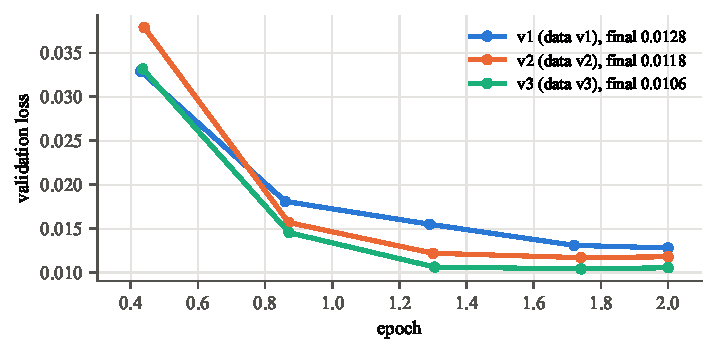
\includegraphics[width=0.72\linewidth]{figures/loss_curves.pdf}
\caption{Validation loss of the all-domains adapters by epoch (each on its own data version's validation set).}
\label{fig:loss}
\end{figure}

% =====================================================================================================================
\section{Results}\label{sec:results}

\subsection{Retrieval}
On a 67-question policy QA set, BM25 retrieval reaches Recall@3 0.967, top-1 0.817, answer-in-context 0.883, covered
when answerable 0.933, current-policy choice 1.00 (old vs.\ new refund policy) and ``not covered'' detection 0.714
(only 7 such questions). The thresholds were tuned on the same set, so these numbers are optimistic.

\subsection{Offline step accuracy}
Table~\ref{tab:offline} compares the untuned base with the tuned versions on the same 267 held-out steps and the same
4-bit MLX stack. Fine-tuning is what makes the small model usable: the untuned model routes 89.1\% of steps correctly
but escalates with 46\% precision and fills tool arguments exactly only 26.8\% of the time. v1 already routed 96.6\%
correctly; every one of its remaining errors involved dates (a date said early in the call had scrolled out of the
6-line context and was never stored, A2 date turns were not escalated, and \cmd{resolve\_date} read ``Friday the
23rd'' as the coming Friday: 69 of 360 spoken forms wrong). Data v2 fixed these in the data and the tools, raising
escalation recall from 65.4\% to 92.3\% and arguments from 90.5\% to 92.5\% (98.4\% in the FastLane configuration).
v3 removed a label bug in A2 (Section~\ref{sec:lessons}): on its own validation set, steps with any error fell from
15 (v2) to 6, and the date the large model says back is carried into the record in 7 of 10 A2 calls (v2: 0 of 10).

\begin{table}[tbp]
\centering\small
\begin{tabular}{@{}lrrrr@{\hspace{2em}}rr@{}}
\toprule
& \multicolumn{4}{c}{267 steps of data v2} & \multicolumn{2}{c}{267 steps of data v3} \\
\cmidrule(r{2em}){2-5}\cmidrule{6-7}
Metric & Untuned & v1 & v2 & & v2 & v3 \\
\midrule
Route accuracy & 89.1 & 96.6 & \textbf{98.9} & & 99.3 & 99.3 \\
Escalation precision & 46.2 & 100 & 96.0 & & 100 & 100 \\
Escalation recall & 23.1 & 65.4 & \textbf{92.3} & & 92.3 & 92.3 \\
Right tool & 49.8 & 96.7 & 96.7 & & 95.9 & \textbf{98.8} \\
Exact tool arguments & 26.8 & 90.5 & \textbf{92.5} & & 97.2 & \textbf{99.0} \\
p50 / p95 latency (s) & 2.20 / 7.55 & 2.22 / 4.83 & 2.22 / 4.51 & & 2.32 / 4.88 & 1.96 / 4.24 \\
\bottomrule
\end{tabular}
\caption{Offline step accuracy (\%) of the small model, same steps and serving stack within each block.}
\label{tab:offline}
\end{table}

\paragraph{Error analysis of v3.} The 6 remaining errors: two changes that call \cmd{modify\_booking} without
searching first, one \cmd{quantity} instead of \cmd{party\_size} in a restaurant change, one extra policy search, one
complaint handed to staff by calling the tool instead of routing (same outcome) and one missed A2 escalation.

\subsection{New domain (RQ3, offline)}
The movies+buses adapter (A8) has never seen a restaurant call. On the 54 restaurant steps of data v2 it routes 98.1\%
correctly (all-domains v2: 100\%; untuned: 87.0\%), with escalation recall 88.9\% (100\%; 33.3\%) and the right tool
88.9\% of the time (95.6\%; 46.7\%). Argument filling does \emph{not} transfer: 47.6\% exact (100\%; 50.0\%), and all
11 errors are the same one, \cmd{quantity} (the movie/bus field) where restaurants need \cmd{party\_size}. The gateway
rejects such calls, so in a live call this costs an extra step or a hand-off. Routing transfers; the schema does not.

\subsection{Pilot: untuned vs.\ tuned small model}
Table~\ref{tab:pilot} compares two 24-call pilots (one call per domain $\times$ category
cell, same calls, same caller simulator and large model); only the small model changed. The tuned model keeps easy
turns: the share of turns sent to the large model falls from 60.7\% to 13.5\%, large-model tokens per call fall
5$\times$, the free-tier rate limit is never hit (110\,s of waiting per call $\rightarrow$ 0), and median model time
per turn falls by 42\%. Success rises from 79.2\% to 87.5\% (policy 0/3 $\rightarrow$ 2/3, sold out and change of mind
2/3 $\rightarrow$ 3/3). Two numbers got worse. \emph{p95} rose because the slowest turns are now booking turns where the
small model takes two steps in a row (search, then read-back: about 3\,s + 5\,s on MLX), plus one 45.6\,s Gemini
reply. \emph{Router recall} fell because the test labels mark every relative date as hard, while FastLane handles
dates on the small model with code tools by design; 5 of the 13 ``missed'' hard turns are such date turns, and those
calls succeeded. The intervals overlap (24 calls, one seed): this is a pilot, not the final comparison.

\begin{table}[tbp]
\centering\small
\begin{tabular}{@{}lrr@{}}
\toprule
24 calls & Pilot v0 (untuned) & Pilot v3 (tuned) \\
\midrule
Task success [95\% CI] & 79.2\% [59.5--90.8] & \textbf{87.5\%} [69.0--95.7] \\
Turns sent to the large model & 60.7\% & \textbf{13.5\%} \\
Large-model calls / tokens per call (in / out) & 6.12 / 12,013 / 1,051 & \textbf{1.04} / \textbf{2,316} / \textbf{200} \\
Rate-limit wait per call & 110.3\,s & \textbf{0\,s} \\
Model time per turn p50 / p95 & 2.88\,s / \textbf{6.89\,s} & \textbf{1.66\,s} / 8.06\,s \\
Router precision / hard-turn recall & 25.3\% / \textbf{90.5\%} & \textbf{76.5\%} / 56.5\% \\
Invalid tool calls & 7.6\% & \textbf{0.9\%} \\
Success with injected tool errors & 100\% & 100\% \\
Unsafe / unconfirmed / rule-breaking writes & 0 / 0 / 0 & 0 / 0 / 0 \\
Missed hand-offs & 0/3 & 0/3 \\
Success by domain (buses / movies / restaurants) & 6/8, 7/8, 6/8 & 5/8, 8/8, 8/8 \\
\bottomrule
\end{tabular}
\caption{24-call pilots with FastLane; only the small model differs (untuned Qwen2.5-3B vs.\ adapter v3).}
\label{tab:pilot}
\end{table}

\subsection{Failures and the fixes they led to}\label{sec:fixes}
All three failed calls of pilot v3 were buses, and all were the small model acting alone where it should not
(Table~\ref{tab:fixes}). No gateway rule was broken, but two calls showed that passenger details were not checked
against what the caller had actually said. The voice demo later showed a related gap (a search with a cinema nobody
named and without the time the caller gave), which led to the grounding rule. Both rules were checked against all 650
generated practice calls: the same 645 calls are kept and \emph{no} training example changes, so the rules never
block a correct booking in our data. After the fixes, the 3 failed calls were rerun and all 3 succeed.

\begin{table}[tbp]
\centering\small
\begin{tabularx}{\linewidth}{@{}lLL@{}}
\toprule
Call & What went wrong & Fix and outcome on rerun \\
\midrule
bus-dates-161 & asked ``Which cinema?'' in a bus call, then booked invented passengers (``Caller (40)'') & passenger-source rule: the booking is refused, the large model asks for both passengers; booked correctly \\
bus-rule\_break-236 & caller asked for 3 seats but gave 1 passenger; model booked 1 seat with an invented age & passenger-count check: two attempts refused, call handed to staff (an accepted outcome) \\
bus-policy-201 & small model misread the refund table (90\% instead of 25\% for 10\,h before departure) & policy answers with numbers go to the large model: answered 25\% \\
mov-sold\_out-056 & one Gemini backup reply took 45.6\,s & backup capped at 20\,s, no retry, lost time counted as waiting \\
\bottomrule
\end{tabularx}
\caption{Pilot v3 failures, the code fixes (no retraining) and the rerun.}
\label{tab:fixes}
\end{table}

\subsection{Baselines and ablations on 24 calls}\label{sec:baselines}
We ran the baselines and ablations on the same 24 calls as the pilots, with adapter v3, the fixes above, the same
caller simulator and the same large model (Table~\ref{tab:baselines}, Figure~\ref{fig:systems}). FastLane, B2, A2 and
A8 ran for the mid-submission; B1, B3 and A3 ran on 6--7 November, after the daily API quota reset and after the
tool-description fix described under B1 below, so they also include the other code fixes of 6 November (count
check, \cmd{party\_size} alias, repeated tool calls passed on); FastLane's row predates them and is rerun with
the same code in the final runs. Each run is one seed; the intervals are wide, so only large gaps are
meaningful.

\begin{table}[tbp]
\centering\footnotesize
\setlength{\tabcolsep}{3.5pt}
\begin{tabular}{@{}lrrrrrrrr@{}}
\toprule
System & Calls & Success [95\% CI] & \hcell{Large-model\\turns} & \hcell{Large calls\\per call} & \hcell{p50 / p95\\(s)} & \hcell{Invalid\\tool calls} & \hcell{Unsafe-\\write calls} & \hcell{Router\\P / R} \\
\midrule
\textbf{FastLane} & 24 & \textbf{95.8\%} [80--99] & 21.3\% & 1.67 & 1.55 / 7.59 & \textbf{0.8\%} & \textbf{0} & \textbf{65} / 77 \\
FastLane, before fixes & 24 & 87.5\% [69--96] & 13.5\% & 1.04 & 1.66 / 8.06 & 0.9\% & 0 & 77 / 57 \\
B1 large only & 24 & 87.5\% [69--96] & 100\% & 8.21 & \textbf{1.17} / \textbf{2.32} & 0.8\% & 6 (+2)$^\S$ & -- \\
B2 untuned small & 24 & 29.2\% [15--49] & 0\% & 0 & 2.12 / 19.74 & 26.1\% & 0 & -- \\
B3 large as router & 24 & \textbf{95.8\%} [80--99] & 72.6\% & 6.25 & 2.14 / 9.92 & 0.9\% & 0 & 48 / 83 \\
A1 no fine-tuning$^\dagger$ & 24 & 79.2\% [60--91] & 60.7\% & 6.12 & 2.88 / 6.89 & 7.6\% & 0 & 25 / \textbf{91} \\
A2 no date tools & 24 & 87.5\% [69--96] & 43.5\% & 3.58 & 2.94 / 7.76 & 2.8\% & 0 & 35 / 87 \\
A3 rules in prompt & 24 & 66.7\% [47--82] & 28.9\% & 2.08 & 2.06 / 9.22 & 5.8\% & \textbf{13} & 39 / 57 \\
A8 movies+buses & 8$^\ddagger$ & 75.0\% [41--93] & 25.0\% & 1.62 & 1.52 / 5.49 & 12.1\% & 0 & 33 / 60 \\
\bottomrule
\end{tabular}
\caption{Baselines and ablations on the 24 pilot calls (one seed). Model time excludes rate-limit waiting. Router
P / R counts date turns as hard; with dates resolved in code (FastLane's design) FastLane's recall is 94\%, B3's 83\%.
$^\dagger$Pilot v0, run before the gateway fixes. $^\ddagger$Restaurant calls only; FastLane succeeds on 7 of the same 8.
$^\S$Plus 2 calls with a duplicate booking, which the metric does not count (see text).}
\label{tab:baselines}
\end{table}

\begin{figure}[tbp]
\centering
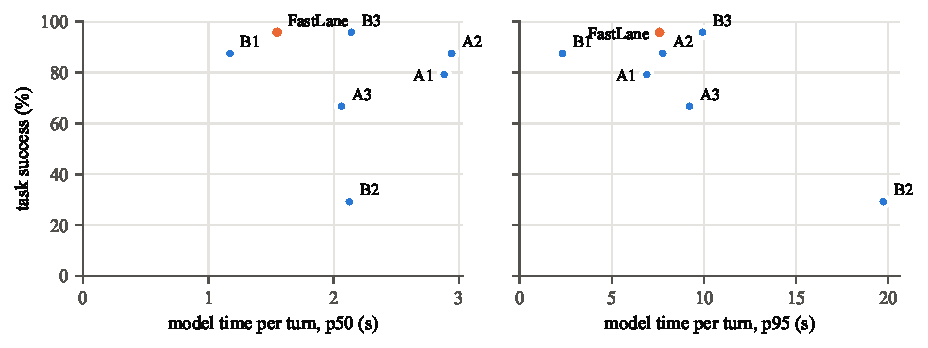
\includegraphics[width=0.92\linewidth]{figures/systems.pdf}
\caption{Task success vs.\ median (left) and p95 (right) model time per turn on the 24 calls. FastLane and B3 have
the highest success; B1 (large model on Groq) has the lowest median and p95 model time.}
\label{fig:systems}
\end{figure}

\paragraph{FastLane.} The fixes of Section~\ref{sec:fixes} lift success from 87.5\% to 95.8\% (23/24); buses
8/8, movies 8/8, restaurants 7/8. It sends more turns to the large model than before the fixes (21.3\% vs.\ 13.5\%)
because numeric policy answers and refused bookings now go there by design. The one failure, res-policy-321, gave the
correct deposit (Rs 2,400), but the simulated caller's next reply was read as a change of mind and the call went to
staff. There were no unsafe writes and no missed hand-offs, and all calls with an injected tool error succeeded.

\paragraph{B1: the large model alone (H1, H2).} With every turn on gpt-oss-120b and the rules in the prompt, B1
succeeds in 21 of 24 calls (87.5\%; FastLane 23/24, intervals overlap). Two failures are duplicate bookings: after
``your booking is confirmed'' the caller said ``yes'' once more and B1 booked again. The third is a wrong bus (22:00
instead of 21:00) after a change of mind. Six more calls contain a write the caller never confirmed: a booking made
as soon as the name was given, and cancellations or changes made in the first turn without a read-back. All six
still ended in the right state, so success alone hides them. FastLane's gateway blocks both patterns, because a
confirmation is used up by one write and any further write needs a new read-back. The unsafe-write metric does not
count the duplicates, because the ``booking confirmed'' message repeats the details and the caller said yes to it. B1
also uses far more of the large model: 8.21 calls and 20.1k tokens per call, against 1.67 calls and 4.4k tokens for
FastLane (78\% fewer tokens). On the free tier (200k tokens a day) that is about 10 B1 calls a day, and B1 waited
19 minutes per call for quota.

B1 is, however, the fastest system: p50 1.17\,s and p95 2.32\,s per turn, against 1.55\,s and 7.59\,s for FastLane. A
single gpt-oss-120b call on Groq takes 0.4--1.4\,s, while one small-model step on the laptop (4-bit MLX) has a median of
1.5\,s. FastLane's slow turns are the 13 of 108 turns that need two small-model steps (median 6.0\,s) and the turns
that are first tried by the small model and then passed on. Without the four turns answered by the Gemini
backup, FastLane's p95 is still 6.6\,s. The proposal assumed that a large API model adds 1--3\,s per turn; on Groq it
adds about 1\,s, so on this setup routing to a local model saves cost, quota and unsafe writes, not time.

\paragraph{B3: the large model as router.} When gpt-oss-120b decides before each turn whether it is hard, B3 matches
FastLane's success (23/24) and, using the same gateway, makes no unsafe writes. But it sends 72.6\% of turns to the large model
(FastLane 21.3\%), makes 6.25 large-model calls per call (3.7$\times$) and adds a router call to every turn, so its
p50 is 2.14\,s and its p95 9.92\,s (7.2\,s without Gemini-served turns). It is also the worse router: with dates
handled in code it catches 83\% of hard turns at 38\% precision, against 94\% at 65\% for the tuned small model. Its
failure (bus-sold\_out-176) ended without the booking.

\paragraph{B2: the untuned small model alone fails.} It succeeds only where the right outcome is a refusal or a
hand-off (red flags 3/3, rule-breaking requests 3/3, returning callers 1/3, every other category 0/3). A quarter of
its tool calls are invalid, it loops through many steps (34.5k prompt tokens per call vs.\ 3.7k for FastLane, 226
turns vs.\ 108), and its p95 is 19.7\,s. A small model can only replace the large model on easy turns once it is tuned.

\paragraph{A1: no fine-tuning.} The untuned small model in FastLane (pilot v0) passes 60.7\% of turns on and makes
6.1 large-model calls per call (FastLane: 1.7), with 79.2\% success. Its p95 (6.9\,s) is below FastLane's because the
large model answers most turns in one step; the cost is 3.7$\times$ the large-model calls and a 110\,s rate-limit wait
per call on the free tier. A1 also predates the gateway fixes, so it differs from FastLane in more than one flag.

\paragraph{A2: no date and alternative tools (H4).} Without \cmd{resolve\_date} and \cmd{find\_alternatives} the
small model cannot handle dates or sold-out shows, so it passes them on: the share of turns sent to the large model
doubles (21.3\% $\rightarrow$ 43.5\%), large-model calls per call rise 2.1$\times$ (1.67 $\rightarrow$ 3.58), large-model
tokens per call rise 1.5$\times$, and median model time per turn rises from 1.55\,s to 2.94\,s. Success falls from
23/24 to 21/24: one wrong date in a change of mind (15 October instead of 23 October), one
booking that was never made, and one policy question handed to staff. A2's router recall looks better (87\% vs.\
77\%) only because it passes almost everything on.

\paragraph{A3: rules only in the prompt, no read-back (H5).} This is the clearest result. With the same models but
no gateway rules and no read-back gate, \textbf{13 of 24 calls made a booking change that the caller never confirmed}
(17 such writes) and 5 writes broke a booking rule; FastLane made none. All 3 rule-breaking calls failed: a
cancellation after the cut-off, a cancellation for a caller whose phone number did not match, and 1 seat booked for a
caller who asked for 3 passengers. Two more bus bookings had passenger names the caller never said. Seven of the 13
calls with unconfirmed writes still ended in the right state, so task success alone (66.7\%) understates the risk:
the rules and the read-back are what make the writes safe. The mid-submission version of this run (15/24 unsafe
calls, 75\% success) used tool descriptions that promised a read-back the ungated gateway never gives; the rerun with
truthful descriptions gives the same conclusion.

\paragraph{A8: new domain end to end (H6).} The movies+buses adapter succeeds on 6 of the 8 restaurant calls
(FastLane 7/8). Half of the calls (4/8) contained one invalid tool call (12.1\% of tool calls vs.\ 0.8\%), the
\cmd{quantity}/\cmd{party\_size} mismatch found offline; the gateway rejected each one and 3 of these 4 calls still
succeeded. The extra failure was a change of mind where the old time (14:00) was kept instead of the new one (12:30).
A8 uses the v2 adapter (the movies+buses adapter was not retrained on data v3), so the gap mixes domain and data version.

\subsection{FastLane after fixing its final-run errors}\label{sec:afterfix}
In the final run on 120 calls (Groq paid tier, gpt-oss-120b only), FastLane succeeded on 108 calls (90.0\%). Reading
all 12 failed transcripts gave 6 simulated-caller failures (mostly no change of mind), 1 scorer failure and 5 agent
errors: a bus origin the caller never said (2 calls), ``Your booking was cancelled'' after the gateway had refused
the cancellation, a ``no parking'' answer that contradicted the retrieved text, and a retrieval miss handed to staff.
We fixed the first three kinds (rows 34--37 of Table~\ref{tab:allfixes}) and reran FastLane on the same 120 calls as
a separate run; the comparison runs were not changed.

\begin{table}[tbp]
\centering\small
\begin{tabular}{@{}lrrrrrr@{}}
\toprule
Run & Success & \hcell{p50 / p95\\per turn (s)} & \hcell{Large\\turns} & \hcell{Large calls\\per call} & Unsafe & \hcell{Failures: caller /\\scorer / agent} \\
\midrule
before fixes & 108/120 (90.0\%) & 1.67 / 6.81 & 20.9\% & 1.76 & 0 & 6 / 1 / 5 \\
after fixes & 105/120 (87.5\%) & 1.66 / 6.62 & 20.5\% & 1.64 & 0 & 7 / 2 / 6 \\
\bottomrule
\end{tabular}
\caption{FastLane on the same 120 calls before and after the fixes of rows 34--37. Failure causes from reading every
failed transcript.}
\label{tab:afterfix}
\end{table}

All four calls that failed through the targeted errors now succeed, and none of the three error types occurs in the
new run: the origin rule refused 9 searches, all in calls where the caller had not named the origin, and the agent
asked instead. Overall success did not rise (Table~\ref{tab:afterfix}): 13 calls changed outcome between the runs,
8 of them with no fix involved, so run-to-run variation (Groq and the simulated caller are not deterministic) is
about $\pm$7\% of calls, and the difference is not significant (paired test, 5 vs 8 calls, $p=0.58$). One ``new''
failure is a correct answer: the large model said the Dal Makhani has no nuts, which the menu confirms, but no accepted
phrase matched; before the fix the small model had said it was \emph{not} nut-free and the scorer accepted that
because ``not nut-free'' contains ``nut-free''. We did not change the scorer after seeing the results. The six agent
errors after the fixes are of other kinds (a stale read-back after a change of mind, twice saying a booking was
``already'' at the newly asked time, ``Which cinema?'' in a bus call, a booking the caller had not asked for, and the
same retrieval miss). The lesson is that single-run differences of a few calls cannot show the effect of a fix; the
transcripts can.

\subsection{Voice pipeline}
\cmd{fastlane voice} serves a browser page; one WebSocket per call carries 16\,kHz audio. Silero VAD ends a turn after
600\,ms of silence and sends partial transcripts every 0.6\,s to early lookup; Whisper large-v3-turbo on MLX
transcribes with a domain word list (film, cinema, branch, city and festival names); the unchanged FastLane agent
replies; Kokoro speaks the reply sentence by sentence. It is half duplex, with a typed-text fallback. We used a small
FastAPI loop instead of Pipecat so that every stage is timed in one trace. In an 8-turn spoken booking (TTS-made
caller) the median times were: STT 1.04\,s, agent 1.3\,s, first reply audio 0.45\,s, and \textbf{3.2\,s from the end
of speech to the first reply audio} (plus the 0.6\,s silence wait). The slowest turn (10.2\,s) was a read-back: two
small-model steps (5.8\,s) and a long first sentence; a short lead-in (``Just to confirm:'') is now spoken as its own
chunk. Live calls exposed three hand-off problems, now fixed in code: the large model said it would transfer the
caller but called no tool (the hand-off is now made in the same turn when a reply announces it), Markdown was read
aloud (replies are converted to plain sentences and lists), and the page hid the end of the call.

\subsection{Speech recognition on Indian English}
Table~\ref{tab:stt} compares recognisers on 300 random clips of the Svarah test split (real speakers with 15+ first
languages, general topics) and on 142 caller lines from the pilots spoken by four Kokoro voices, two of them
Hindi-accented. Key-detail accuracy is the share of places, films, names and numbers in the reference that appear in
the transcript after normalisation. Sarvam is best on real Indian speech by a wide margin and 3$\times$ faster
(best or near-best for every first-language group, e.g.\ Kannada 7.0\% vs.\ 11--43\%). The domain word list helps only
in domain: it lifts places on booking lines from 48\% to 97\% but raises WER on Svarah's general speech by 3--4
points. Person names are the weak spot for every recogniser (26--37\%). We also found and fixed a setting of ours:
Whisper had been run with temperature fixed at 0, which disables its fallback decoding and let short clips fall into
repetition loops (turbo + word list: 20.1\% WER before, 14.9\% after).

\begin{table}[tbp]
\centering\small
\begin{tabular}{@{}lrr@{\hspace{2em}}rrrr@{}}
\toprule
& \multicolumn{2}{c}{Svarah (300 clips)} & \multicolumn{4}{c}{Booking lines, TTS (142 clips)} \\
\cmidrule(r{2em}){2-3}\cmidrule{4-7}
Recogniser & WER & s / clip & WER & Places & Names & Numbers \\
\midrule
Sarvam saarika:v2.5 (cloud) & \textbf{5.8} & \textbf{0.46} & 8.1 & 80.6 & \textbf{36.8} & 96.7 \\
Whisper large-v3-turbo (MLX) & 10.5 & 1.42 & 9.4 & 48.4 & 26.3 & 95.8 \\
\quad + domain word list & 14.9 & 1.40 & 8.0 & \textbf{96.8} & 26.3 & 94.2 \\
faster-whisper small.en (CPU) & 9.5 & 1.34 & 10.8 & 48.4 & 26.3 & \textbf{97.5} \\
\quad + domain word list & 12.3 & 1.50 & \textbf{7.8} & \textbf{96.8} & 26.3 & \textbf{97.5} \\
\bottomrule
\end{tabular}
\caption{Speech recognition: WER (\%), median time per clip, and key-detail accuracy (\%) on booking lines.}
\label{tab:stt}
\end{table}

\subsection{Speech noise in training data}\label{sec:noise}
Since data v1, about 30\% of training steps have a copy whose caller lines are rewritten by hand-made rules
(``Kukatpally'' $\rightarrow$ ``kuka pally'', ``four'' $\rightarrow$ ``for'') with the same target. Measured on the
1,762 caller lines of data v4, \textbf{14.9\% of these rule-based copies lose a key detail that the target still
contains} (e.g.\ ``for tickets'' with target \cmd{quantity: 4}), which teaches the model to fill in values nobody said;
a live call did exactly that (a misheard ``Authenticates'' read back as 4 tickets). Data v5 replaces the rules with a
round trip: every caller line, twice, is spoken by a Kokoro voice (half Hindi-accented, speed 0.9--1.15), passed
through a phone channel (300--3400\,Hz, noise at 12--30\,dB SNR) and transcribed by the same Whisper set-up the voice
demo uses. A transcript is used only if every key detail survives (places, films, dates, names, numbers, booking
references, short forms such as ``Oct''/``Hyd'', and yes/no polarity, since ``Haan \dots na'' heard as ``maybe not''
must not become a yes). Of 3,524 clips (mean WER 35.7\%, median 20\%), 55.7\% are usable; names are lost most often
(1,334 clips), then numbers (335).

To see how much recogniser noise hurts the current model, we ran v3 on the 245 validation steps of data v4 once
with clean caller lines and once with usable round-trip transcripts (192 steps changed). Routing is unaffected
(98.8\% vs.\ 98.8\%; escalation recall 88.5\% both; right tool 96.3\% vs.\ 96.8\%), but exact arguments fall from
\textbf{98.1\% to 94.3\%}. The new errors are the kind the round-trip copies target: twice ``8:30 PM'' was transcribed
as ``8th, 30 p.m.'' and v3 searched for 18:00, a time nobody said; a party of 5 was searched as 2; ``on the bus?''
became ``on the back?'' and a policy search went to restaurants. Data v4 and v5 contain the same calls and differ only
in the noise copies, which makes them a clean ablation once both are trained.

\paragraph{Adapter v5 (trained 7 November).} Both adapters were trained on data v5 (eval loss 0.0113 all-domains,
0.0161 movies+buses). On the same 245 steps, v5 routes better (escalation recall 96.2\% vs.\ 88.5\%) and loses less
under recogniser noise: exact arguments fall from 95.9\% to 94.8\% (v3: 98.1\% to 94.3\%), and where v3 invented
18:00 from ``8th, 30 p.m.'', v5 leaves the time out and asks. On clean text its arguments are 2 steps worse, and it
sometimes replies where it should search. End to end on the 24 calls with the same code, v3 and v5 both succeed in
21/24, but v3 catches more hard turns (93.8\% vs.\ 78.6\%), has fewer invalid tool calls (1.6\% vs.\ 5.0\%) and a
lower p95 (6.8 vs.\ 9.5\,s), and v5 made the only failure caused by the agent (it took a policy question about
cancelling for a cancellation request). The other failures came from the simulated caller (it did not change its
mind, or booked against its goal), which costs 2--3 of 24 calls per run. FastLane therefore keeps v3 for the
typed-text final runs; v5 is the noise ablation and the better model for the voice demo. The v5 run also exposed two
gaps, now fixed in code: a policy figure given with no policy search now goes to the large model, and the large
model's backup now also takes over when the primary is unreachable, not only when it is rate-limited.

% =====================================================================================================================
\begin{table}[tbp]
\centering\small
\begin{tabularx}{\linewidth}{@{}>{\raggedright\arraybackslash}p{3.7cm}>{\raggedright\arraybackslash}p{3.3cm}L@{}}
\toprule
Hypothesis & Expected & Evidence so far \\
\midrule
H1 Routing is faster & p95 $\geq$50\% lower than B1 & \textbf{not supported} on this setup: B1 on Groq p50 1.17\,s / p95 2.32\,s, FastLane 1.55 / 7.59\,s; the local small model is slower per step than the hosted large model. FastLane uses 78\% fewer large-model tokens \\
H2 Quality holds & within 3 points of B1 & \textbf{supported} (24 calls): FastLane 95.8\% vs.\ B1 87.5\%, intervals overlap; B1 also has 8 calls with unconfirmed or duplicate bookings \\
H3 Router catches hard turns & $\geq$90\% passed on & \textbf{supported}: 94.4\% end to end with dates resolved in code (77.3\% if date turns count as hard); B3 83.3\%; offline 92.3\% \\
H4 Tools cut large-model use & clearly lower with tools & \textbf{supported}: without the tools (A2) large-model turns 21.3\% $\rightarrow$ 43.5\%, calls per call 1.67 $\rightarrow$ 3.58, success 23/24 $\rightarrow$ 21/24 \\
H5 Rules in code are safer & fewer unsafe writes & \textbf{supported}: rules in the prompt only give 13/24 unsafe calls and 5 rule-breaking writes (A3), and 6/24 plus 2 duplicate bookings with the large model (B1); FastLane 0 \\
H6 Routing transfers & within 5 points on restaurants & offline routing 98.1\% (vs.\ 100\%), arguments 47.6\% (field mismatch); end to end 6/8 vs.\ 7/8 restaurant calls (one call = 12.5 points) \\
H7 Early lookup hides delay & lower p95 on lookup turns & not shown: in the 24-call run 9 lookups started, 2 reused, 3 wasted, negligible time saved \\
\bottomrule
\end{tabularx}
\caption{Hypotheses of the proposal and the evidence so far.}
\label{tab:hyp}
\end{table}

\section{Challenges Faced and Mitigation}\label{sec:lessons}

\paragraph{Challenges already solved.} Every retraining and fix so far was driven by an observed failure;
Table~\ref{tab:history} summarises the chain. Three lessons
generalise. (1) \emph{Most model errors came from the data, not from training}: every v1 error traced back to how
dates were represented, and v2's A2 errors to labels that could not be learned (the date the large model said back was
never written into the record, so after it scrolled out of the context the target date was invisible). (2)
\emph{Check that a new model is really new}: the first v2 evaluation reproduced v1 exactly because a stale merged
folder was reused; the merge now always starts from scratch and every build is checked by weight hash. The same
lesson recurred on Kaggle, where a run meant for v4 trained the old dataset version (Table~\ref{tab:runs}).
(3) \emph{Safety belongs in code}: no FastLane run produced an unsafe write, when the small model invented
passengers or a cinema a gateway rule stopped it without retraining, and A3 and B1 show what happens without
these rules (13 and 6 of 24 calls with unconfirmed writes). (4) \emph{A baseline must not inherit the system's
wording}: the first B1 run booked twice in each of its first three calls, because the ungated tools still said
``the first call returns a read-back'' while it already booked; ungated systems now get truthful descriptions.

\begin{table}[tbp]
\centering\small
\begin{tabularx}{\linewidth}{@{}lLL@{}}
\toprule
Where & Challenge & Mitigation (done) \\
\midrule
Pilot v0 & untuned model sends 61\% of turns to the large model; refund-rule questions go to staff & fine-tune (data v1, adapter v1) \\
Adapter v1 & all remaining errors involve dates (context loss, A2, weekday bug) & data v2: dates as slots resolved in code; \cmd{resolve\_date} fix \\
Adapter v2 & first check identical to v1 & stale merge folder; merge from scratch, hash check \\
Adapter v2 & A2 date labels unlearnable; 5 wrong A2 dates & data v3 and adapter v3 (A2 carries the ISO date) \\
Scoring & ``October 24'' scored wrong against 2026-10-24 & dates compared by day; saved rows rescored \\
Pilot v3 & invented passengers, partial booking, misread refund table & passenger-source rule, numeric policy answers to the large model \\
Voice demo & details dropped from long openings; unrequested cinema & data v4 (multi-detail openings); grounding rule \\
STT on Svarah & repetition loops on short clips & restore Whisper's temperature fallback \\
Rule noise & 14.9\% of noise copies contradict their target & data v5: TTS$\rightarrow$STT round trip with a key-detail filter \\
Live calls & announced but unmade hand-offs; Markdown read aloud & same-turn hand-off; plain-speech replies \\
Mid runs & Groq daily token cap (200k) and the Gemini backup's free tier ran out during the runs & resumable runner kept every finished call; waits excluded from model time; B1, B3 run after the mid-submission \\
B1 run & double bookings: ungated tools described a read-back that never came & truthful tool descriptions when rules are off; B1 and A3 rerun, old files kept \\
Mid-run errors & count from a misheard word; \cmd{quantity} for a table (A8); same tool call repeated 4 times & ticket/party count must have been said; field alias; repeated call goes to the large model at once \\
\bottomrule
\end{tabularx}
\caption{Challenges met so far and how each was resolved (details and evidence files are in the run log).}
\label{tab:history}
\end{table}

\paragraph{Open challenges and mitigation plans.} Table~\ref{tab:risks} lists the challenges that still affect the
final results and how we plan to handle them before 15 November.

\begin{table}[tbp]
\centering\small
\begin{tabularx}{\linewidth}{@{}>{\raggedright\arraybackslash}p{3.9cm}LL@{}}
\toprule
Challenge & Impact & Mitigation plan \\
\midrule
Large-model rate limits (Groq free tier: 200k tokens/day; a B1 call uses $\approx$20k) & about 10 B1 calls a day; the 24-call B1/A3/B3 runs took 34\,h; backup model (Gemini, 4--7\,s per call) mixes latencies & paid tier or a second key for the final runs; otherwise FastLane and B1 on 72 calls, the rest on 24--48; waiting logged apart from model time; report which model answered \\
Little time left to the final submission & 12 systems $\times$ 360 calls $\times$ 3 seeds will not fit & stratified subsets (above), one seed \\
p95 latency (small model 1.5\,s per step; two steps on booking turns) & H1 not supported against B1 on Groq & report the trade-off honestly (cost, quota, safety vs.\ time); repeated tool calls now go to the large model at once; speculative decoding with a 0.5B draft model if time allows \\
Names misheard by every recogniser (26--37\% exact) & wrong passengers, failed bookings in voice calls & the read-back lists every name for the caller to confirm, so errors are not silent; spelling names back deferred (it changes the trained dialogue flow) \\
New-domain arguments (A8: \cmd{quantity} vs.\ \cmd{party\_size}) & A8 calls fail on the schema, not on routing & field alias in the gateway (done, 6 Nov); A8 rerun with the alias, reported separately from routing \\
Simulated callers may be unrealistic & success rates may not transfer to real callers & 20 real team calls and 30 transcripts checked against simulated ones \\
Kaggle runs used a stale dataset version once & lost a 3.5\,h run & check data sizes in the notebook before leaving it to run; weight hashes for every build \\
\bottomrule
\end{tabularx}
\caption{Open challenges and mitigation plans for the final submission.}
\label{tab:risks}
\end{table}

% =====================================================================================================================
\section{Status of the Hypotheses}\label{sec:status}

Table~\ref{tab:hyp} states what the evidence so far says about each hypothesis. The ablations support H4 (code
tools for dates and alternatives halve the large-model share) and H5 (rules and read-back in code remove unconfirmed
and rule-breaking writes). Against the large model alone (B1), FastLane holds quality (H2: 95.8\% vs.\ 87.5\%) with
78\% fewer large-model tokens and no unsafe writes, but H1 fails: gpt-oss-120b on Groq answers faster (p95 2.3\,s)
than the laptop-hosted 3B model (p95 7.6\,s). Against a large model used as router (B3), FastLane has the same success
with a third of the large-model calls and lower latency, and its router catches more hard turns (H3: 94\% vs.\ 83\%).
So RQ1 is answered in part: routing to a tuned small model keeps quality and cuts large-model use, but it cuts time
only when the large model is slower than the local one. H6 holds for routing but not for tool arguments, and H7 has
no support yet. All of this rests on 24 calls with one seed.


\section{Remaining Work and Timeline to the Final Submission}\label{sec:todo}

The final submission is due on 15 November 2026. Table~\ref{tab:timeline} gives the plan: the first two rows are
done, the rest is planned. Since H1 is not supported against B1 on Groq, the final runs focus on what does separate
the systems: success, unsafe writes and large-model use, on more calls.

\begin{table}[tbp]
\centering\small
\begin{tabularx}{\linewidth}{@{}>{\raggedright\arraybackslash}p{2.0cm}L>{\raggedright\arraybackslash}p{3.6cm}@{}}
\toprule
Dates & Work & Output \\
\midrule
30 Oct & mid-submission; FastLane, B2, A2, A3, A8 on 24 calls & mid report (done) \\
31 Oct--7 Nov & code fixes: heard-count check, \cmd{party\_size} alias, repeated tool call to the large model, truthful tool descriptions without rules, router recall with dates in code (196 tests; training data v5 unchanged by them); B1, B3 and A3 rerun on 24 calls & Table~\ref{tab:baselines} complete (done) \\
8--9 Nov & train data v5 on Kaggle (both adapters); offline check of v5 vs.\ v3; 24-call check of v5 and v3 with the new code; two more fixes (203 tests) & FastLane keeps v3; v5 is the noise ablation (done) \\
9--12 Nov & final runs, one seed: FastLane and B1 on a stratified 72-call subset (120 with a paid API tier), B3, A2, A3, A8 on 48 calls & success, unsafe writes, large-model use with 95\% intervals \\
9--12 Nov (in parallel) & two team members label 300 turns (Cohen's $\kappa$); real team calls; voice runs with Sarvam STT & $\kappa = 0.17$ between annotators, 0.65 / 0.42 against the rule (Table~\ref{tab:kappa}, done); real-call check, end-to-end latency \\
13--14 Nov & analysis of H1--H7 and RQ1--RQ3; error analysis; figures; final report, README, demo video & results section \\
15 Nov & code freeze on GitHub & final submission \\
\bottomrule
\end{tabularx}
\caption{Timeline from the mid-submission to the final submission (15 November 2026).}
\label{tab:timeline}
\end{table}

\paragraph{If time runs short.} The conversion of Schema-Guided Dialogue and Taskmaster-1 into training data and the
spelled-back names (which would change the dialogue flow the adapter was trained on) are dropped first. Without a
paid API tier, B1 costs about 20k large-model tokens per call against 4.4k for FastLane, so the B1 run is the one
that limits the plan: it stays, and the other systems shrink to the 24-call runs already done.

\section{Limitations and Safety}
All results so far come from synthetic callers, a practice booking system and at most 24 end-to-end calls with one
seed; apart from B2 and A3, the confidence intervals of all systems overlap. The large model is a free-tier model with
a backup, so its latency varies, and the latency comparison depends on the hardware: the small model runs on a laptop
and the large model on Groq's inference hardware. The round-trip noise uses synthetic voices, which are harsher than Svarah's real speech in places
and softer in others. The routing labels come from rules that two annotators without a written guideline did not
agree on ($\kappa = 0.17$, Table~\ref{tab:kappa}); a model trained on them learns one design's policy, not a
shared human judgement. On safety, the system follows the proposal's plan: a mock system only, no payment tool,
read-back before any change, identity check by phone number, hand-off with a summary for complaints, payments and
out-of-scope requests, and an agent that states it is automated. All test callers are synthetic; API keys stay in a
local environment file and are never logged.


\end{document}
